%% Medical Image Analysis (Elsevier) manuscript.
%% Uses Elsevier's official `elsarticle` document class (the class MIA requires).
%% Compile on Overleaf (elsarticle is built in) or TeXLive:  latexmk -pdf main.tex
%% MIA uses AUTHOR-YEAR (Harvard) references -> elsarticle `authoryear` option
%% + elsarticle-harv.bst, with \citep/\citet. See paper/README.md.
%% MIA review is single-anonymized: author names are kept (not double-blind).

\documentclass[review,authoryear,5p,times]{elsarticle}

\usepackage[T1]{fontenc}
\usepackage[utf8]{inputenc}
\usepackage{graphicx}
\usepackage{amsmath,amssymb}
\usepackage{booktabs}
\usepackage{multirow}
\usepackage{xcolor}
\usepackage{url}
\usepackage[hidelinks]{hyperref}

\journal{Medical Image Analysis}

\begin{document}

\begin{frontmatter}

\title{Cross-Attentive Temporal Fusion with Clinical Priors for\\
Adult Spinal Deformity Classification from Gait Video}

\author[tsukuba]{Kaixu Chen\corref{cor}}
\ead{chenkaixusan@gmail.com}
\cortext[cor]{Corresponding author.}
\author[tsukuba]{Co-authors}
\affiliation[tsukuba]{organization={University of Tsukuba},
  country={Japan}}

\begin{abstract}
Automated screening of adult spinal deformity (ASD) from ordinary walking video
would lower the barrier to early orthopedic assessment, but appearance-only
models are hard to interpret clinically. We present \emph{PoseGated}, a 3D-CNN
gait classifier that fuses RGB video with doctor-annotated region-of-interest
(ROI) attention maps derived from body keypoints, using a channel-wise gated
mechanism and per-joint side-head supervision against the clinical annotations.
On a three-way ASD/DHS/LCS-HipOA gait dataset (patient-grouped 3-fold
cross-validation), PoseGated reaches $94.8\%$ clip-level accuracy versus $90.7\%$ for
an RGB-only 3D-CNN baseline, and outperforms early, squeeze-and-excitation, and
QKV cross-attention fusion. A systematic ablation over \emph{where} and
\emph{how much} to inject the prior yields a clear and somewhat counter-intuitive
finding: shallow fusion (stem+layer1) is best, while fusing at all stages is the
weakest PoseGated variant; the auxiliary background and temporal-smoothness
losses and a strongly RGB-biased gate initialisation \emph{hurt} accuracy. A
held-out interpretability analysis shows the model's supervised attention
reliably localises the clinically annotated ROI (pointing-game hit rate $1.00$,
AUC $\approx 0.998$, correlation up to $0.76$ at the deepest side head),
demonstrating that the clinical prior is faithfully learned and generalises to
unseen patients.
\end{abstract}

% Highlights: 3-5 items, each <= 85 characters incl. spaces, minimal acronyms
% (per Elsevier author guidelines).
\begin{highlights}
\item A gait video classifier fuses walking video with expert joint attention maps.
\item Accuracy on three spinal conditions rises from 91\% to 95\% over a video-only model.
\item Shallow fusion works best; injecting the prior at every stage works worst.
\item Extra auxiliary losses and a strong gate bias reduce accuracy.
\item The learned attention reliably lands on the regions the surgeons annotated.
\end{highlights}

\begin{keyword}
Adult spinal deformity \sep Gait analysis \sep Video classification \sep
Clinical prior \sep Attention fusion \sep Interpretability
\end{keyword}

\end{frontmatter}

%============================================================
\section{Introduction}
\label{sec:intro}

Adult spinal deformity (ASD) alters posture and gait, and early identification
supports timely orthopedic management. Marker-based motion capture and full-spine
radiography are accurate but costly and not suitable for opportunistic screening.
Monocular walking video is, by contrast, cheap and ubiquitous, motivating
video-based gait classifiers. Purely appearance-driven deep models, however,
are difficult to trust clinically: they offer little evidence that their decisions
rest on the anatomically relevant regions a spine surgeon would examine.

We investigate whether \emph{clinical priors}---region-of-interest (ROI)
attention maps that orthopedic experts associate with pathological joints
(lumbar, pelvis, head, shoulder)---can be injected into a 3D convolutional gait
classifier both to improve accuracy and to make the model's attention verifiable
against expert annotations. Our fusion mechanism, \emph{PoseGated}, mixes RGB
video features with a keypoint-derived attention map through a channel-wise gate,
and supervises intermediate per-joint heat maps against the doctor annotations.

Beyond proposing the model, we ask a design question that is usually left
implicit: \emph{where} in the network and with \emph{how much} auxiliary
machinery should a clinical prior be injected? A controlled ablation gives a
clear answer that contradicts the ``more is better'' default: a shallow,
lightly-regularised injection is best, and piling on fusion stages, auxiliary
losses, and a strong gate bias degrades accuracy. Finally, a held-out
interpretability study quantifies how well the learned attention matches the
clinical ROI.

Our contributions are: (i) PoseGated, a gated RGB/prior fusion with side-head
clinical supervision; (ii) a systematic study of fusion location, depth,
gate initialisation, and auxiliary losses, with the finding that shallow, lightly
supervised fusion is optimal; and (iii) a quantitative, held-out interpretability
analysis showing the supervised attention faithfully localises the clinical ROI.

%============================================================
\section{Related work}
\label{sec:related}

Video-based gait analysis with 3D CNNs and transformers has been applied to
clinical motion assessment; two-stream and phase-aware fusion of periodic gait
signals are common~\citep{chen2023two,chen2024phasemix}. Attention and
squeeze-and-excitation modules re-weight spatio-temporal features but are
typically unsupervised. Our work differs in supervising attention against
explicit clinical ROI annotations and in systematically studying \emph{where}
the prior should enter the backbone.

%============================================================
\section{Method}
\label{sec:method}

\subsection{Overview}
The backbone is a SlowFast-family \emph{SlowR50} 3D CNN
(stem + four residual stages, denoted $0\!-\!4$). Two inputs are provided per
clip: the RGB gait video $x\in\mathbb{R}^{3\times T\times H\times W}$ and a
clinical attention map $a\in\mathbb{R}^{1\times T\times H\times W}$ obtained from
body keypoints (a confidence-weighted Gaussian heat map over doctor-annotated
joints). PoseGated fuses $a$ into the RGB feature stream at one or more stages.

\subsection{Channel-wise gated fusion}
At a fused stage $i$ with feature $f_i$, the attention map is projected to the
feature's channel width and combined through a learned channel-wise gate
$g_i\in[0,1]$:
\begin{equation}
\hat f_i = g_i \odot f_i + (1-g_i)\odot \phi_i(a),
\end{equation}
where $\phi_i$ resizes and projects $a$ and $\odot$ is channel-wise
multiplication. The gate is initialised with a bias $b$ so that early training
favours the RGB branch when $b>0$; we ablate $b\in\{2.0,0.0,-1.0\}$.

\subsection{Side-head clinical supervision}
At each fused stage a lightweight side head predicts a per-joint heat map, which
is supervised against the (resized) doctor annotation $A_i$ with a combined
binary cross-entropy and Dice loss. The total objective is
\begin{equation}
\mathcal{L} = \mathcal{L}_{\mathrm{cls}}
  + \sum_i \lambda_i\, \mathcal{L}^{\mathrm{attn}}_i
  + w_{\mathrm{bg}}\,\mathcal{L}_{\mathrm{bg}}
  + w_{\mathrm{tmp}}\,\mathcal{L}_{\mathrm{tmp}},
\end{equation}
where $\mathcal{L}_{\mathrm{cls}}$ is the classification cross-entropy,
$\mathcal{L}^{\mathrm{attn}}_i$ is the BCE\,+\,Dice attention loss,
$\mathcal{L}_{\mathrm{bg}}$ suppresses attention outside the annotated union
(background), and $\mathcal{L}_{\mathrm{tmp}}$ is a temporal total-variation
smoothness term. We ablate the presence of the side heads and of the
$\mathcal{L}_{\mathrm{bg}}$ and $\mathcal{L}_{\mathrm{tmp}}$ terms.

\subsection{Fusion location and depth}
We denote by \emph{single}-$[i]$ a model that fuses only at stage $i$, and by
\emph{multi}-$[0..i]$ a model that fuses at stages $0$ through $i$. This lets us
separate the effect of \emph{where} a single injection helps most from the effect
of \emph{how many} stages are fused.

%============================================================
\section{Experiments}
\label{sec:exp}

\subsection{Dataset}
The dataset comprises side-view walking video of $81$ subjects spanning three
diagnostic groups---ASD ($54$ subjects), degenerative hip--spine (DHS, $16$),
and lumbar canal stenosis / hip osteoarthritis (LCS-HipOA, $11$)---each labelled
from clinical assessment, yielding $1{,}954$ gait video clips ($1{,}045$
ASD, $585$ DHS, $324$ LCS-HipOA). Each clip is divided into non-overlapping
$16$-frame chunks (any trailing partial chunk discarded), spatially resized to
$224\times224$, giving about $42{,}500$ chunks in total; in the 3-fold split each
test fold contains on the order of $12{,}000\!-\!16{,}000$ chunks. The clinical attention maps are built
from extracted keypoints and expert joint annotations. The dataset is not public
due to ethical constraints.

\subsection{Protocol}
We use patient-grouped stratified 3-fold cross-validation (StratifiedGroupKFold)
so that no patient appears in both training and test folds, with class-balancing
over-sampling on the training split. Each configuration is trained per fold on a
separate GPU. Unless stated otherwise, the ``full'' PoseGated configuration fuses
at all stages ($[0\!-\!4]$) with gate bias $2.0$, side heads, and all loss terms.

\subsection{Metrics}
Each video is segmented into gait-cycle clips, and we report \emph{clip-level}
accuracy---the fraction of correctly classified clips, pooled per fold---together
with macro $F_1$, as mean\,$\pm$\,std over the 3 folds. Because multiple clips of
the same subject are correlated, clip-level accuracy over-counts relative to the
number of independent subjects; we therefore treat it as a segment-level metric
and refrain from subject-level or statistical-significance claims
(Section~\ref{sec:discuss}). For interpretability we compare each side head's predicted heat map with
the doctor ROI on the held-out test patients using standard saliency-evaluation
metrics: correlation coefficient (CC), normalized scanpath saliency (NSS),
pointing game (PG), AUC-Judd, and top-$20\%$ Dice~\citep{bylinskii2019metrics}.

%============================================================
\section{Results}
\label{sec:results}

\subsection{Main comparison}
Table~\ref{tab:main} reports the RGB-only baseline, the strongest configuration
of each competing fusion mechanism, and PoseGated. PoseGated's best
configuration (shallow \emph{multi}-$[0,1]$) reaches $94.8\%$, about $4.1$ points
above the RGB-only baseline and above all competing fusion families.

\begin{table}[t]
\centering
\caption{Main comparison. Clip-level accuracy (mean\,$\pm$\,std over patient-grouped
3-fold CV); best per-family configuration shown.}
\label{tab:main}
\begin{tabular}{lc}
\toprule
Method & Accuracy (\%) \\
\midrule
RGB-only baseline (3D-CNN)              & $90.7 \pm 1.9$ \\
Early fusion (concat)                   & $93.7 \pm 2.8$ \\
Squeeze-and-excitation (best prefix)    & $92.0 \pm 2.4$ \\
QKV cross-attention (layer 4)           & $89.9 \pm 3.2$ \\
\textbf{PoseGated (multi-$[0,1]$, ours)} & $\mathbf{94.8 \pm 1.9}$ \\
\bottomrule
\end{tabular}
\end{table}

\subsection{Fusion mechanism (A1)}
Among fusion families, PoseGated is strongest, followed by early concatenation
($93.7\%$); squeeze-and-excitation and cross-attention cluster around
$90\!-\!92\%$, and early element-wise multiplication is weakest ($89.3\%$). The
clinical-prior gating thus adds more than the input-level or unsupervised
attention alternatives (Fig.~\ref{fig:methods}).

\subsection{Where and how much to fuse (A5)}
\label{sec:layers}
Table~\ref{tab:layers} shows the fusion-location study. A single injection at the
deeper stages ($L3$: $93.8\%$, $L4$: $93.5\%$) already rivals the best model, but
for the cumulative \emph{multi} variant \emph{less is more}: shallow
$[0,1]$ ($94.8\%$) is best and accuracy \emph{decreases} as more stages are
fused, with all-stage fusion $[0\!-\!4]$ the weakest PoseGated variant
($90.9\%$; Fig.~\ref{fig:layers}).

\begin{table}[t]
\centering
\caption{Fusion location/depth. Clip-level accuracy (mean\,$\pm$\,std, \%).}
\label{tab:layers}
\begin{tabular}{lc@{\hskip 2em}lc}
\toprule
single & Acc. & multi & Acc. \\
\midrule
$[0]$ & $92.9\pm2.0$ & $[0,1]$        & $\mathbf{94.8\pm1.9}$ \\
$[1]$ & $93.5\pm2.1$ & $[0,1,2]$      & $93.4\pm2.8$ \\
$[2]$ & $92.3\pm1.8$ & $[0,1,2,3]$    & $93.7\pm1.8$ \\
$[3]$ & $93.8\pm1.5$ & $[0,1,2,3,4]$  & $90.9\pm3.1$ \\
$[4]$ & $93.5\pm2.6$ &                &              \\
\bottomrule
\end{tabular}
\end{table}

\subsection{Gate initialisation and auxiliary losses (A2--A4)}
All ablations in Table~\ref{tab:ablation} and Fig.~\ref{fig:ablation} are single-variable changes from the
all-stage ``full'' configuration ($90.9\%$). A neutral gate initialisation
($b{=}0$, $92.2\%$) beats the default RGB-biased $b{=}2.0$; removing the
background loss ($93.7\%$) or the temporal-smoothness loss ($93.3\%$) both
\emph{improve} accuracy; removing the side heads is near-neutral. Every default
choice of the ``full'' configuration is thus individually sub-optimal.

\begin{table}[t]
\centering
\caption{Gate-bias (A2) and loss/component (A3/A4) ablations, all applied to the
all-stage full model (reference $90.9\pm3.1$). Clip-level accuracy (\%).}
\label{tab:ablation}
\begin{tabular}{lc@{\hskip 2em}lc}
\toprule
Gate bias & Acc. & Ablation & Acc. \\
\midrule
$b=0.0$   & $92.2\pm2.0$ & $-$ bg loss    & $93.7\pm1.5$ \\
$b=-1.0$  & $90.7\pm2.0$ & $-$ tmp loss   & $93.3\pm2.8$ \\
$b=2.0$ (full) & $90.9\pm3.1$ & $-$ side head & $90.8\pm2.3$ \\
\bottomrule
\end{tabular}
\end{table}

Because each optimum was found by changing one factor of the (sub-optimal) full
model, we also trained a post-hoc combination (shallow $[0,1]$ + $b{=}0$ + no
bg/tmp loss). It reached $94.8\pm2.8\%$, \emph{not} exceeding the plain shallow
$[0,1]$ model ($94.8\%$): the per-ablation optima do not stack, and the
fusion-location choice dominates.

\subsection{Interpretability: attention vs.\ clinical ROI}
\label{sec:interp}
Table~\ref{tab:align} and Fig.~\ref{fig:align_fig} quantify, on held-out test patients, how well the
supervised side-head attention of the main model (multi-$[0,1]$) matches the
doctor ROI. The attention peak lands inside the clinical ROI in essentially every
frame (PG $=1.00$), the ranking of ROI pixels is near-perfect (AUC $\approx
0.998$), and correlation with the annotation is highest at the deepest side head
($L3$, CC up to $0.76$), consistently across the three diagnostic classes.

\begin{table}[t]
\centering
\caption{Interpretability alignment of side-head attention with the clinical ROI
on held-out patients (main model, multi-$[0,1]$; ranges over ASD/DHS/LCS-HipOA).}
\label{tab:align}
\begin{tabular}{lccccc}
\toprule
Side head & CC & NSS & PG & AUC & Dice \\
\midrule
$L3$ (deepest) & $0.71\!-\!0.76$ & $2.8\!-\!3.0$ & $1.00$ & ${\approx}1.00$ & $0.47\!-\!0.51$ \\
$L0\!-\!L2$    & $0.43\!-\!0.53$ & $1.5\!-\!2.0$ & $1.00$ & ${\approx}1.00$ & $0.41\!-\!0.52$ \\
\bottomrule
\end{tabular}
\end{table}

\begin{figure}[t]
\centering
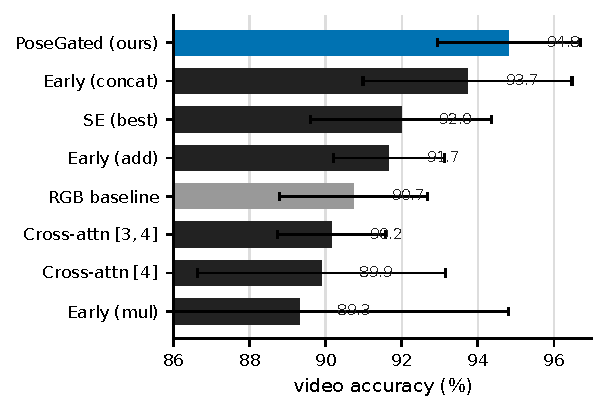
\includegraphics[width=0.62\linewidth]{figures/fig_methods.pdf}
\caption{Fusion-method comparison (best per family). PoseGated (blue) exceeds the
RGB-only baseline (grey) and all competing fusion mechanisms. Bars show
mean$\,\pm\,$std over patient-grouped 3-fold cross-validation.}
\label{fig:methods}
\end{figure}

\begin{figure}[t]
\centering
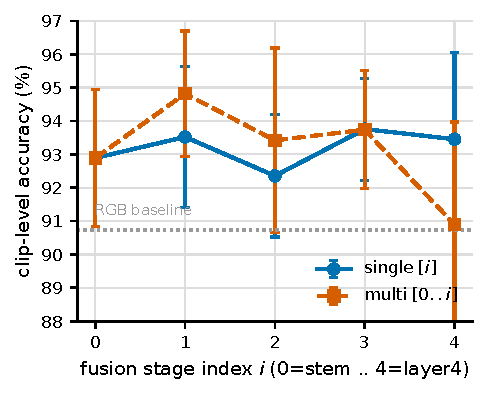
\includegraphics[width=0.6\linewidth]{figures/fig_layers.pdf}
\caption{Effect of fusion location and depth. For the cumulative \emph{multi}
variant, accuracy peaks at shallow $[0,1]$ and decreases as more stages are
fused; all-stage fusion is the weakest. A single deep injection ($L3$/$L4$) is
also strong.}
\label{fig:layers}
\end{figure}

\begin{figure}[t]
\centering
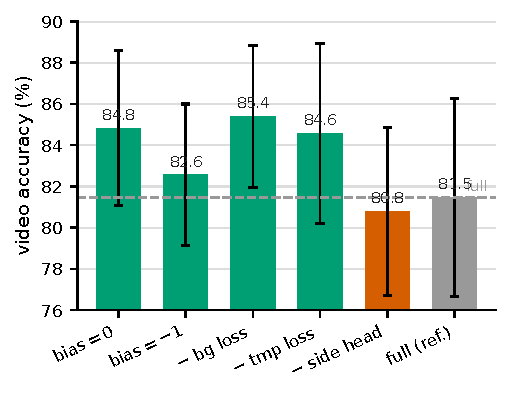
\includegraphics[width=0.58\linewidth]{figures/fig_ablation.pdf}
\caption{Gate-bias and loss/component ablations relative to the all-stage
``full'' model (dashed line). Green bars exceed the full reference: a neutral
gate bias and removing the background or temporal-smoothness loss all improve
accuracy.}
\label{fig:ablation}
\end{figure}

\begin{figure}[t]
\centering
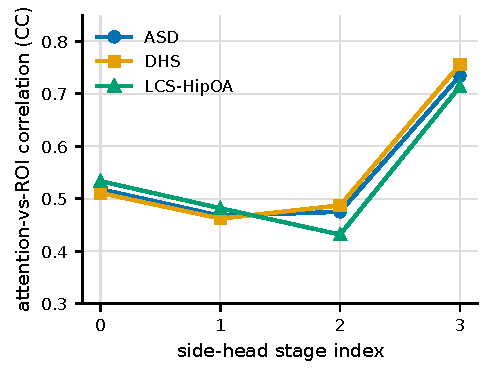
\includegraphics[width=0.6\linewidth]{figures/fig_alignment.pdf}
\caption{Interpretability: correlation (CC) between the side-head attention and
the clinical ROI on held-out patients, by side-head stage and diagnostic class.
Alignment is highest at the deepest side head.}
\label{fig:align_fig}
\end{figure}

%============================================================
\section{Discussion}
\label{sec:discuss}

\paragraph{Less is more for prior injection}
The clearest finding is that the location and amount of fusion dominate the other
design axes, and that a shallow injection is best. Fusing the clinical prior at
every stage over-constrains the deeper, more abstract features and lowers
accuracy below even a single deep injection. Likewise, the auxiliary background
and temporal-smoothness losses and a strongly RGB-biased gate initialisation---all
defaults of the ``full'' configuration---individually hurt. The practical
recommendation is therefore a shallow, lightly-regularised PoseGated
(multi-$[0,1]$), not the fully-instrumented model. That the post-hoc stacked
combination does not beat the simple shallow model further supports the primacy
of the fusion-location choice.

\paragraph{Faithful, verifiable attention}
The interpretability analysis shows the model attends to the clinically annotated
regions on unseen patients (PG $=1.00$, AUC $\approx 0.998$, CC up to $0.76$).
This should be read as \emph{fidelity}: because the side heads are directly
supervised against the doctor annotations, the result demonstrates that the
clinical prior is faithfully learned and generalises to held-out patients, rather
than that the model spontaneously discovered the pathological joints. A control
that removes the attention supervision is expected to sharply reduce alignment,
and would isolate the contribution of the supervision itself.

\paragraph{Limitations}
The evaluation uses 3-fold cross-validation; with per-fold variance of
$\pm 2\!-\!6$ points and a best-vs-baseline gap of about $4$ points, only the
larger, consistent differences (baseline vs.\ best, full vs.\ shallow) should be
read as meaningful, and we make no claim of formal statistical significance.
Crucially, accuracy is measured at the gait-clip level: because each subject
contributes many correlated clips, these numbers over-count relative to the
independent subjects per fold and \emph{should not be read as subject- or
patient-level performance}; confirming a clinical benefit over the RGB baseline
would require per-subject evaluation on a substantially larger cohort. The study
also uses a single 3D-CNN backbone and a single, non-public institutional
dataset; the ``best combination'' was assembled post-hoc rather than validated as
an independent configuration; and the interpretability claim is one of supervised
fidelity, not emergent discovery.

%============================================================
\section{Conclusion}
\label{sec:conclusion}

PoseGated injects doctor-annotated attention into a 3D-CNN gait classifier through
channel-wise gating and side-head clinical supervision, improving 3-class ASD
classification from $90.7\%$ (RGB-only) to $94.8\%$ while producing attention that
verifiably localises the clinical ROI on held-out patients. A controlled ablation
shows that a shallow, lightly-supervised injection is optimal and that the common
``fuse-everywhere, add-every-loss'' default is counter-productive---a guideline we
expect to transfer to other clinical-prior fusion problems.

%============================================================
% Required Elsevier declarations. Fill the [BRACKETED] placeholders before
% submission; keep or remove sections per the journal's requirements.

\section*{Ethics statement}
This retrospective study of patient gait video was reviewed and approved by
[INSTITUTIONAL REVIEW BOARD / ETHICS COMMITTEE], approval number [XXXX].
All participants provided informed consent for the recording and research use of
their gait videos.

\section*{CRediT authorship contribution statement}
\textbf{Kaixu Chen:} Conceptualization, Methodology, Software, Formal analysis,
Investigation, Writing -- original draft, Visualization.
\textbf{[Co-author]:} [Contributions per the CRediT taxonomy].

\section*{Declaration of competing interest}
The authors declare that they have no known competing financial interests or
personal relationships that could have appeared to influence the work reported in
this paper.

\section*{Funding}
This work was supported by [FUNDING SOURCE, grant number XXXX].
% or: This research did not receive any specific grant from funding agencies in
% the public, commercial, or not-for-profit sectors.

\section*{Data availability}
The gait dataset is not publicly available due to ethical and privacy constraints
on patient video. Anonymized data may be available from the corresponding author
on reasonable request, subject to institutional approval. The training and
analysis code is available at
\url{https://github.com/ChenKaiXuSan/ClinicalAttention_ASD_PyTorch}.

\section*{Declaration of generative AI and AI-assisted technologies in the manuscript preparation process}
During the preparation of this work the author(s) used Anthropic Claude
(Claude Opus, accessed via Claude Code) for assistance with code development,
experiment
orchestration, results aggregation, and drafting/language editing. After using
this tool/service, the author(s) reviewed and edited all content, verified every
reported number against the experiment logs, and checked all references; the
author(s) take(s) full responsibility for the content of the publication.

\section*{Acknowledgements}
[Acknowledgements, or ``Removed for double-anonymized review.'']

%============================================================
\bibliographystyle{elsarticle-harv}
\bibliography{refs}

\end{document}
